\chapter{Fabrication of Coded Illumination Devices}\label{ch:fabrication}

In this chapter, we explore the design and fabrication of microscopes which employ coded illumination and describe the design process for coded illumination devices used in this dissertation. Illumination sources vary significantly between microscope setups based on applications, capabilities, availability, and cost. Early microscope sources involved using a candle or oil lamp for illumination. As early as 1665, Hooke used an oil lamp and water-filled globe to focus an oil lamp onto a sample to be imaged using his early microscope~\cite{hookeMicrographica}. These methods (along with gas lamps) were used for centuries, until the carbon arc-lamp enabled electronic illumination in the late 1800s. Around this time, K\"ohler provided a more complete understanding of proper illumination collection to avoid imaging the source directly onto the sample~\cite{kohler1893neues}, which was widely adopted and continues to be used today (including this work). As new lamp sources were invented (such as the Xenon arc lamp~\cite{anderson1951xenon}, tungsten lamp~\cite{edison1880electric}) they found use in microscopy under the K\"ohler configuration.

The rise of the fluorescent microscope led to the development of light sources with engineered spectral properties, which were designed to have sharp (temporally coherent), non-overlapping excitation and emission spectra and high source power. Spatially coherent sources were used to provide phase contrast \cite{smithDIC, zernike1942phase} by filtering spatially incoherent lamps using a pinhole aperture. With the invention of the laser~\cite{schawlow1958infrared}, spatially and temporally coherent illumination could be directly created and used at high power, improving the SNR of both coherent methods and florescence imaging. This high degree of coherence also leads to artifacts arising from random diffraction off of dust and edges in the optical system, limiting its use for wide-field brightfield microscopy.

Illumination using light-emitting diodes (LEDs) has emerged as an energy-efficient and low-cost alternative to lamp-based sources. As more diverse and efficient semiconductor materials have been discovered, LED light sources have found greater usage for both fluorescence and brightfield imaging. In addition, arrays of LEDs have been used to achieve even greater light throughput~\cite{albeanu2008led}, improve sectioning in confocal microscopy~\cite{poher2007optical}, and provide brightfield and darkfield contrast as well as 3D digital refocusing~\cite{Zheng2011}. When paired with computation, LED arrays have found significant usage for quantitative phase imaging~\cite{tian2015quantitative, phillips2015multi, chen2018quantitative}, super-resolution imaging~\cite{Zheng2013, Tian2014}, and high-throughput imaging~\cite{Ma:15}. These devices have found widespread usage within the computational imaging community due to their simple and low-cost implementation, fast switching, and relatively high light output. However, conventional LED arrays suffer from low light-throughput at high angles due to the angular emission profile of the sources and the large distances between the LED and sample.

In this chapter, we detail the design process and manufacture of several LED array designs and discuss their performance in relevant use-cases and applications described in the previous chapters of this dissertation.

\section{Domed Illumination Devices for Coded Illumination}

Designing the ideal LED array source for optical microscopy is challenging, both in design and manufacture. Several early implementations of the LED array microscope use a planar off-the-shelf LED array such as the $32\times 32$ LED unit available from Adafruit~\cite{Zheng2013, Zheng2011}. While these arrays are inexpensive and widely available, they have limited angular illumination range, low light throughput, and introduce flickering artifacts due to their electronic design. For high-angle high-speed FPM, a more specialized LED array becomes necessary. As shown in~\cite{phillips2015multi, Dominguez:14}, a domed illuminator provides significantly higher intensity at high-NA compared to a planar array. For a planar array, intensity at the sample $I$ can be related to the angle of illumination $\theta$ of the emitter by the equation:

\begin{equation}
    I_{\theta} \propto {\cos(\theta)}^4
\end{equation}

\noindent where $\theta$ is the angle between the illumination vector and the optical axis. When the LEDs are arranged in a domed shape, reducing the intensity falloff to:

\begin{equation}
I_{\theta} \propto {\cos(\theta)}^1
\end{equation}

\begin{figure} [ht]
\begin{center}
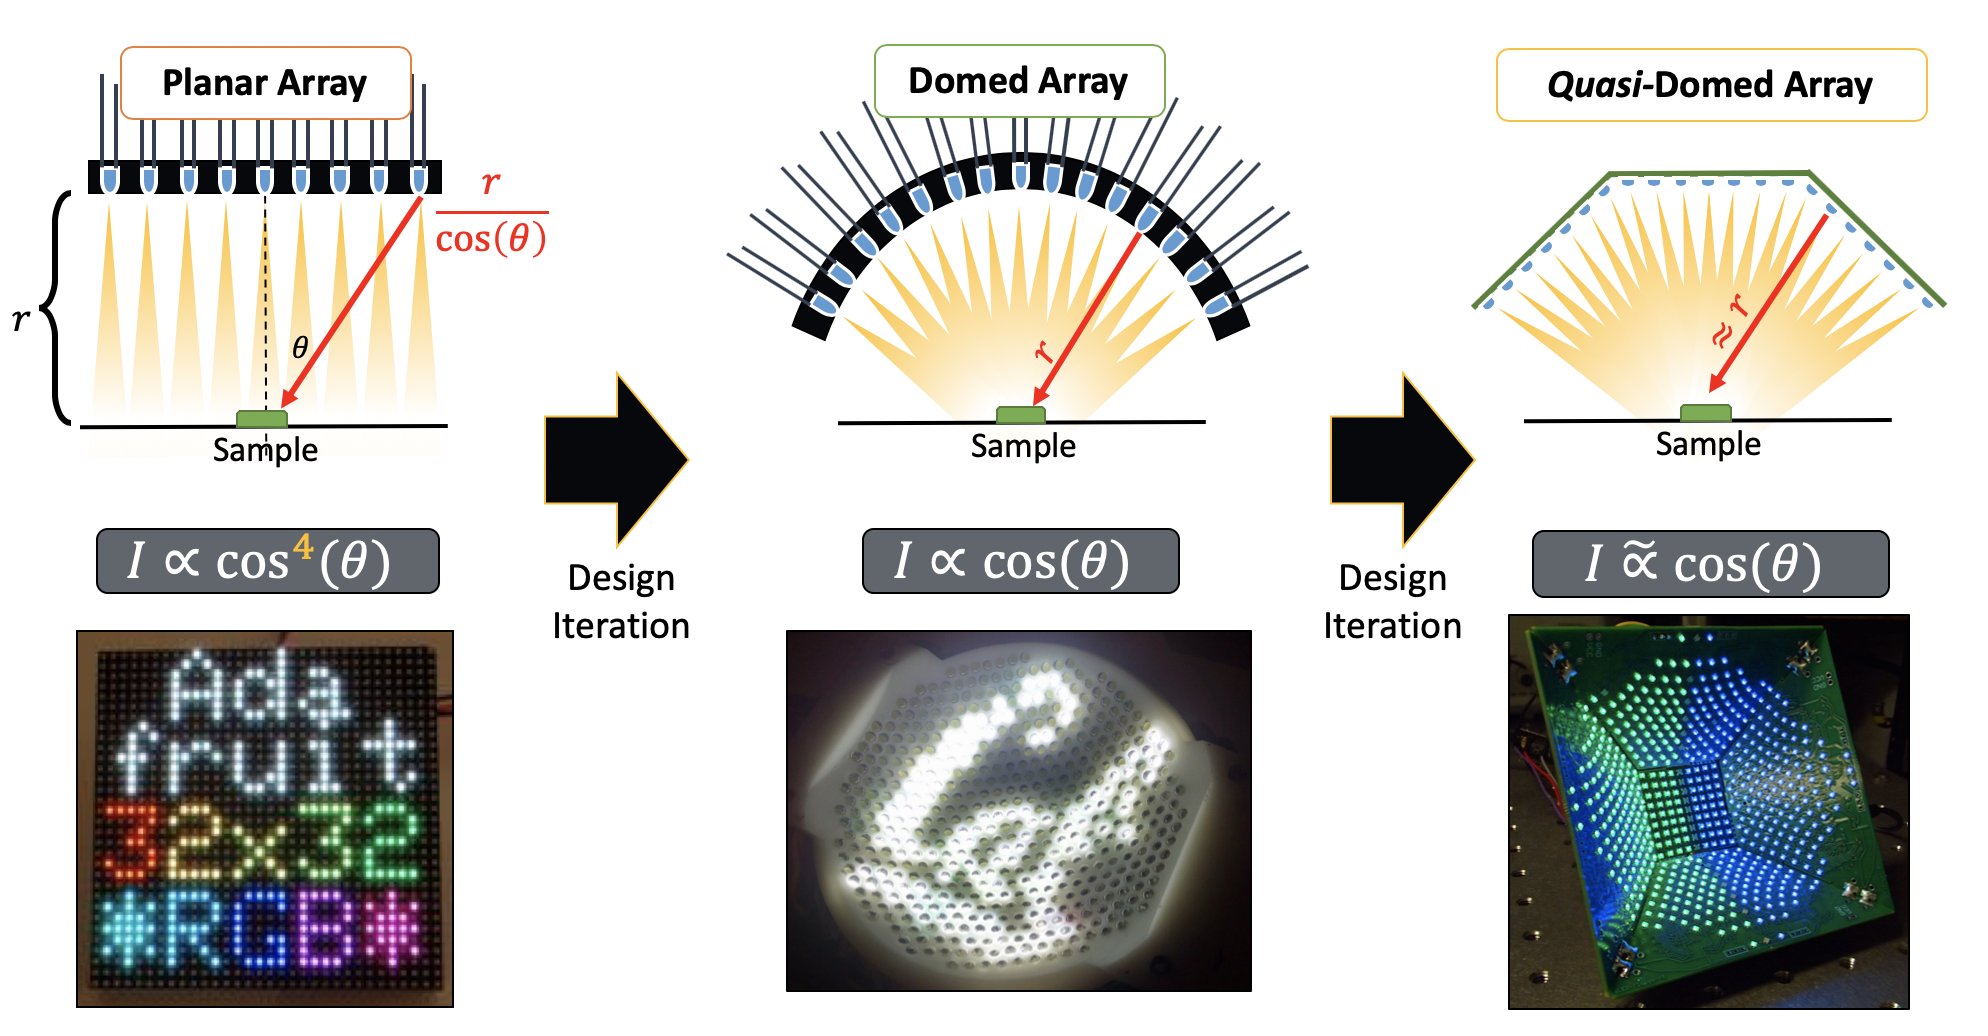
\includegraphics[width=\textwidth]{figures/fig_dome_overview.png}
\end{center}
\caption {Overview of dome designs from the Adafruit 32$\times$32 planar LED array to the proposed quasi-domed device. Our first iteration used a true domed geometry, increasing illumination power at high angles, but was very difficult to fabricate. A second iteration led to the quasi-domed array, which uses standard printed circuit board fabrication processes to make the dome easy to fabricate while maintaining the benefits of a domed geometry.}
\label{fig:fabrication:dome_overview}
\end{figure}

The illumination throughput benefits are a result of two phenomena, shown in Fig. ~\ref{fig:fabrication_ccs_dome}e. The first is that off-axis LEDs in a planar array will have a larger LED-to-sample distance and thus decreased intensity at the sample. For example, if we assume that each LED is a point emitter, the intensity falloff due to increased distance can be expressed as $I(\theta) = I_0 \cos^2(\theta)$, where $I_0$ is the intensity at the sample from the on-axis LED and $\theta$ is illumination angle. The second improvement in light efficiency comes from the fact that LEDs have significant angular variation in intensity (typically emitting more light in the forward direction). In a planar array, the LEDs at higher angles provide less effective illumination, a problem corrected by the dome geometry, where all LEDs are radially oriented. In both the domed and planar geometries we note that intensity further decreases with a final factor of $\cos(\theta)$ due to the smaller profile of objective window when viewed off-axis; combining these factors and assuming a Lambertian ($\sim\cos(\theta)$) angular dependence for physical (non-point-source) LEDs results in an expected intensity falloff of $\sim\cos^4(\theta)$ for the planar geometry but only $\sim\cos(\theta)$ for the domed geometry, a vast improvement at high incidence angles. Thus, the difference between geometries is proportional to $\cos^{3}(\theta)$, or a factor of $> 50 \%$ at 40 degree and $99\%$ at 77-degree incidence, having a substantial impact on illumination throughput, and therefore required exposure times to achieve a good SNR.

In most planar arrays (such as the Adafruit $32 \times 32$ array used in early work~\cite{Zheng2013, Zheng2011}), LEDs are uniformly spaced in Cartesian coordinates across a planar circuit board. When the LED positions are projected onto numerical aperture (NA) coordinates this spacing becomes tighter at high-angles, leading to an uneven sampling across the full range of illumination angles. While having a tighter spacing is usually not a problem for computational imaging applications such as differential phase contrast or Fourier ptychography, it is inefficient, and may lead to unnecessarily long acquisition times. Using a domed geometry is more amenable to creating a uniform LED pattern in angle (NA coordinates) due to geometry and will maintain the LED directionality at high LED angles.

The minimum LED spacing depends on the application. In Fourier Ptychography, for example, early work~\cite{Zheng2013, Tian14, Guo:15} indicated that at least a 60\% pupil overlap ($0.4 \times NA_{objective}$) was necessary in order to properly recover the complex field at high resolution. This quantity depends on the diameter of the pupil (and therefore numerical aperture of the objective); systems with smaller, low-NA objectives will have tighter requirements on LED spacing. The 60\% overlap requirement is developed to provide at least 2$\times$ redundancy of information to reconstruct both amplitude and phase from intensity measurements. Increased overlap beyond this requirement may provide a benefit in terms of SNR, but this effect is difficult to quantify due to the non-linear algorithm used for Fourier ptychographic reconstructions. For DPC-based methods (See chapter~\ref{ch:phase}) LED spacing is naturally restricted to less than the objective NA, since only brightfield LEDs are used. The primary consideration for DPC sources is having LEDs which illuminate at $NA \approx NA_{objective}$ for maximum phase contrast at low-frequencies.

While an LED dome is clearly necessary for obtaining high illumination intensity at high angles, practical limitations on manufacturing and assembly of non-planar circuit boards make building these domes at low cost and large scale non-trivial. In the following sections, we detail the design of a domed LED illuminator through several iterations of the design and prototyping process.

\subsection{3D-Printed Approach}\label{sec:fabrication:ccsdome}

% Dome design figure
\begin{figure} [ht]
\begin{center}
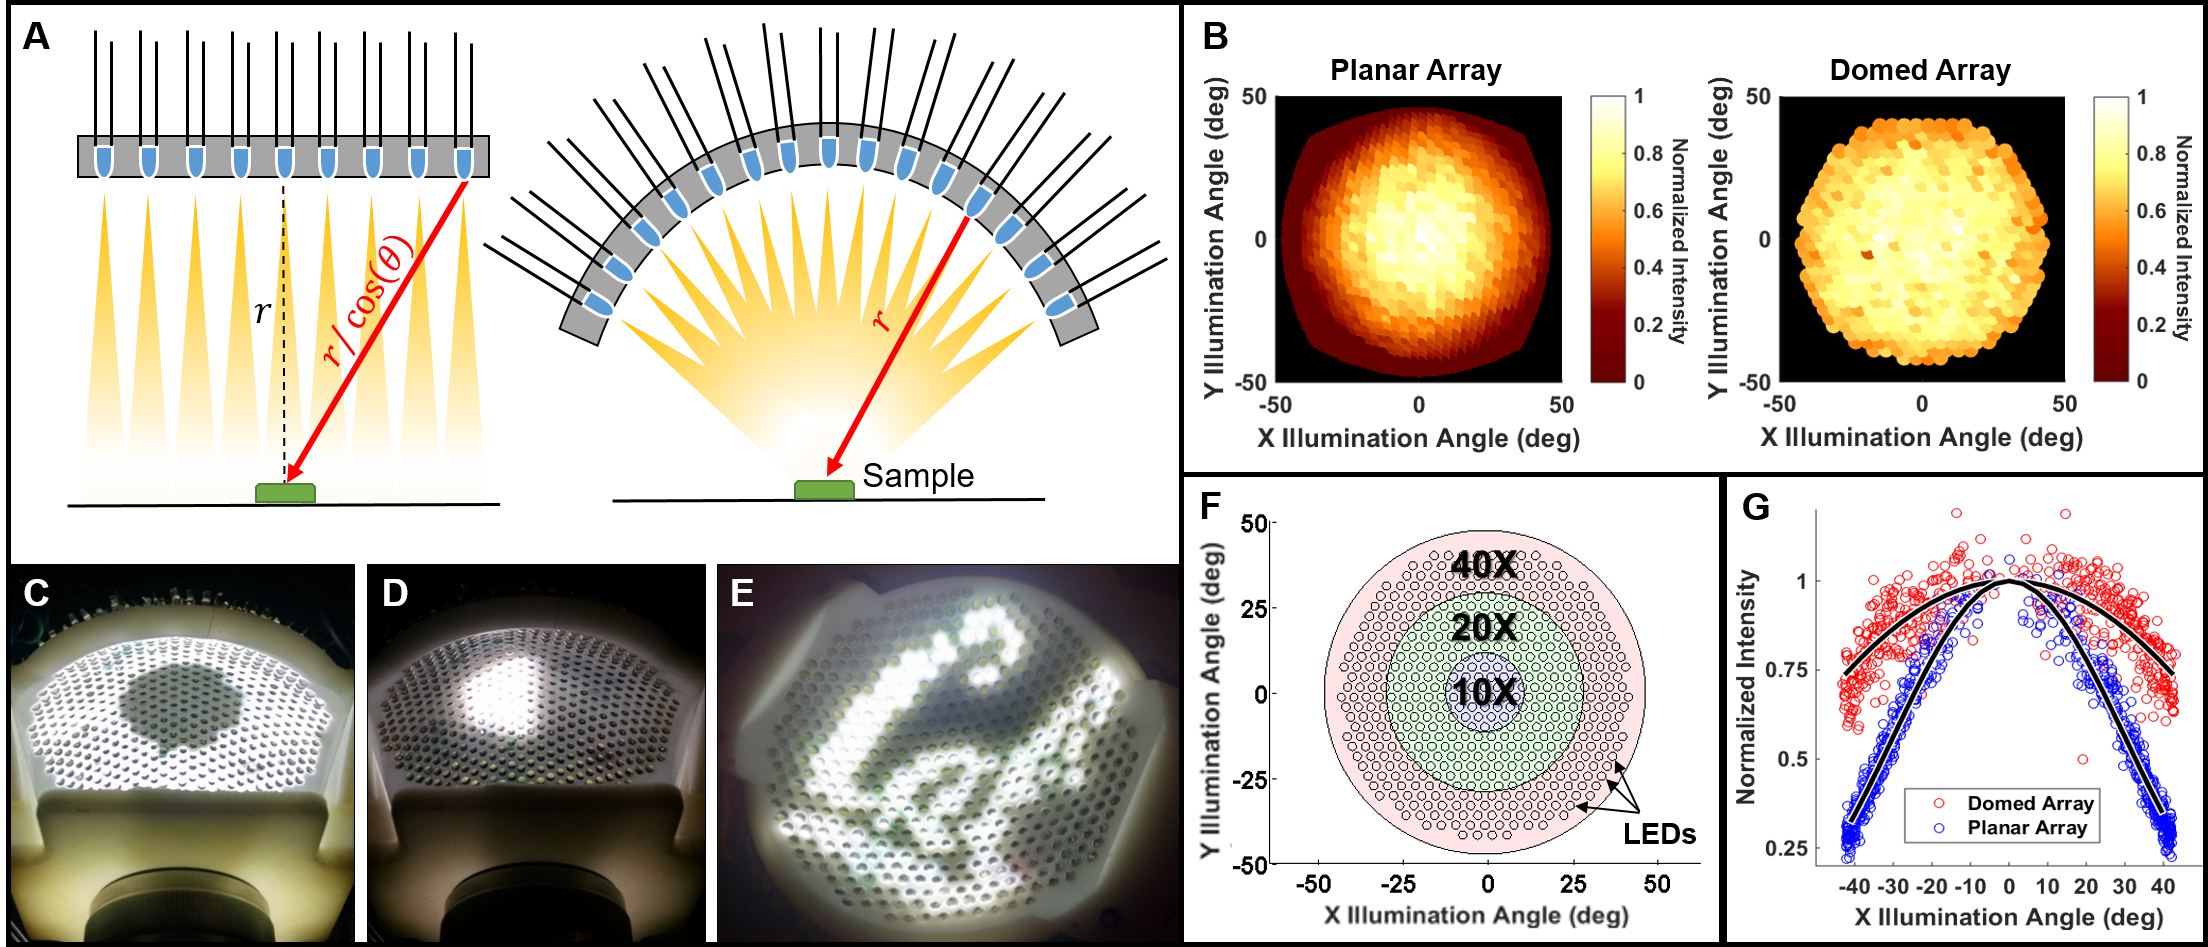
\includegraphics[width=\textwidth]{figures/fig_ccs_dome.png}
\end{center}
\caption {{ Domed LED Illuminator.}
{(a)} Visual comparison of a planar LED array with a domed array. Since the intensity of a spherical wave drops as a function of the inverse square of radius, the illumination at the sample depends on the distance between the LEDs and the sample. In the planar case (left), LED distance $r$ increases as a function of illumination angle, causing weaker illumination at higher angles. A domed LED array (right) eliminates this variation ($r$ is constant).
{(b)} Normalized mean pixel intensities measured at the sensor for the planar and domed arrays. Intensity decreases as a function of angle in both cases, but much more strongly in the case of the planar geometry. Values were normalized to the central LED's brightness in both cases.
{(c)} Illumination pattern used to acquire darkfield images with a 0.25 NA objective.
{(d)} Illumination pattern used to generate differential phase contrast images with a 0.25 NA objective.
{(e)} Illustration of the arbitrary illumination patterning capabilities of the device.
{(f)} Plot illustrating the relative objective NA for several common magnifications, as compared to our dome's LED placement (small black circles).
{(g)} Normalized measured intensity falloff as a function of angle relative to the optical axis for the domed and planar LED arrays. Falloff is proportional to $\cos(\theta)$ for the domed geometry and $\sim\cos^4(\theta)$ for the planar geometry. Black lines are $\cos(\theta)$ and $\cos^4(\theta)$ fits for the domed and planar geometries, respectively.
}
\label{fig:fabrication_ccs_dome}
\end{figure}

The first iteration of domed illuminators was heavily inspired by the AWARE gigapixel camera series~\cite{brady2012multiscale, marks2014characterization, llull2015characterization}, where hundreds of individual cameras were manually inserted into an aluminum dome which enforced opto-mechanical constraints on directionality and position through a hexagonal camera packing. With this inspiration, we designed and fabricated a 3D-printed domed illuminator consisting of 508 individually addressable broad spectrum (white) LEDs uniformly distributed across a domed surface. This first-generation device consists of 4 major components: a hemispherical dome frame for mounting the LEDs, the LEDs themselves, controller circuit boards and the sample stage. The dome mounting structure is a rigid hemisphere designed to constrain the individual LEDs within an array of computationally positioned bores, aligning the LED with the radius vector to the sample center. This hemisphere was designed with a $60 mm$ radius in order to provide maximum intensity at the sample, given our desired number of LEDs and a minimum distance between neighboring LEDs. To pack these LEDs, we used a hexagonal packing pattern across a 77-degree cone of angles with maximum $NA_{illumination} = 0.62$.

The dome hemisphere scaffold was 3D printed (InterPro Models) to achieve the necessary 100$\mu$m printing resolution for accurate LED positioning. The LED angular positions were computed algorithmically to ensure uniform spacing across the dome, constrained by a minimum 150$\mu$m distance between bores for mechanical rigidity and a maximum angular separation of 3.85 degrees allowing for sufficient coherence area at the sample. This angular spacing means that 38 LEDs make up the brightfield region for a common low-NA objective (4$\times$ / $0.1 NA$), with even more for larger NA objectives, ensuring high quality digital refocusing results across a large range of depth slices for all objectives. The $3\textrm{mm}$ through-hole, white LEDs (Mouser 593-VAOL-3LWY4) were press fit into the dome and a rigid lateral constraint was provided by acrylic retaining inserts behind each individual LED. 508 of these LEDs were soldered directly to controller boards arranged above the array, with insulated leads to prevent electrical shorting.

Accounting for mechanical tolerances of the 3D printed dome and the LED epoxy lenses, manufacturing tolerances suggest that the maximum angular pointing error will be no greater than $\pm$4.8 degrees. This corresponds to a maximum intensity attenuation of only 1.2\% due to assembly variation and tolerances across all illumination angles. Our illumination is also quite uniform across the field of view. The maximum field of view of our optical system has a radius of $1.25\textrm{mm}$, set by the eyepiece field-stop diameter of $10\textrm{mm}$ and assuming a 4$\times$ objective. Given the $60\textrm{mm}$ radius of curvature of our dome, this corresponds to illumination variation due to mechanical tolerances being less than 1\% across the field of view for each single LED illumination.  While this result is quite good, the spread of intensities between different LEDs is significantly larger (see Fig.~\ref{fig:fabrication_ccs_dome}g), as a result of combined mechanical, electrical, and parts tolerances. Conveniently, a one-time calibration sweep of illumination angles, taken with no sample present, is sufficient to allow computational removal of this variation for all practical purposes.

The device used nine identical printed circuit boards placed in a fanned arrangement above the dome, each containing four LED controller chips (Texas Instruments TLC5926) serving up to 64 LEDs. These were controlled by a single Arduino Micro micro-controller, which calculates the appropriate bit pattern based on serial commands from an included Bluetooth transceiver. The array is fully addressable through a standard Bluetooth serial link or USB interface. We operate the serial output at 115K baud and note that we can update the entire pattern with approximately 100ms latency, although we predefine some of the more complex LED illumination patterns and store them in the Arduino flash memory to further improve acquisition time. Thus, our acquisition times are primarily limited by the camera rather than the LED array control.

The dome's power control board is tolerant of voltages between 7 and 20 VDC to allow compatibility with a large range of power sources, including a standard 12V automotive battery and a 100W wall-plug variable output power supply, as well as many commercially available portable power supplies for consumer electronics. During regular usage, the device requires no more than 2A of current, though it could potentially draw up to 4.8A of current when all LEDs are illuminated. This is not a typical use case, however, since simultaneous illumination inside and outside the objective NA amounts to an undesirable mixing of darkfield and brightfield contrast. Noting that for 4$\times$, 10$\times$, and 20$\times$ objective configurations there are more darkfield than brightfield LEDs, to reduce power consumption we perform darkfield illumination by default using an annulus with a width equivalent to 0.15NA rather than using all of the darkfield LEDs. This moderately reduces the contrast and resolution of darkfield images but significantly reduces power use during the darkfield illumination cycle. We note that the device can operate indefinitely without overheating issues for both multi-contrast and digital refocusing under normal use.

The completed prototype is shown in Fig.~\ref{fig:fabrication_ccs_dome}. Overall, this prototype was very difficult to manufacture because LEDs had to be inserted by hand, and the leads of each LED had to be manually soldered to one of the 9 circuit boards above the dome. This 3D reconstruction process required significant time and effort to ensure all of the LEDs were functional. The designs of this illuminator were published publicly, but to our knowledge there were no successful reproductions, owing to the difficult fabrication process.

\subsection{Quasi-Dome}\label{sec:fabrication:quasidome}

\begin{figure}
    \centering
    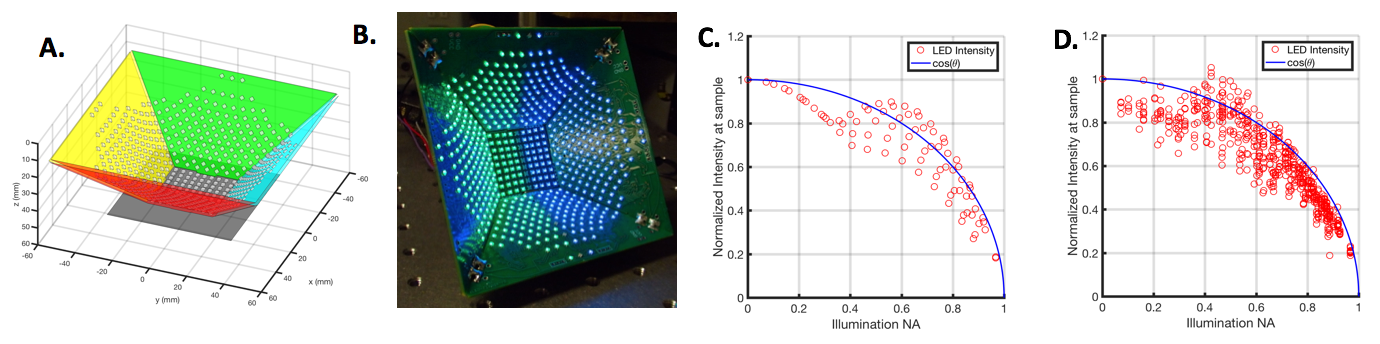
\includegraphics[width=\textwidth]{figures/fig_qdome_main.png}
    \caption{Quasi-dome programmable LED illuminator. (a) CAD model of LED flange positions. (b) Assembled LED array quasi-dome displaying two half circles (center line of LEDs are turned off). (c) Simulated intensity falloff of LED array considering all factors (normalized). (d) Experimental normalized intensity falloff.}\label{fig:fabrication:fig_fabrication_quasi_dome}
\end{figure}

In response to difficulties experienced in fabricating the 3D-printed dome, we developed a quasi-domed LED array consisting of 5 panels (see Fig.~\ref{fig:fabrication:fig_fabrication_quasi_dome}a,b), each of which are standard printed circuit boards (PCBs) with all components pre-assembled using standard manufacturing techniques. This domed illuminator used multi-channel LEDs (Knightbright APTF1616 series) which have individual channel control without multiplexing using on-board LED controllers (Texas Instruments TLC5955), connected in a serial daisy-chain (Fig.~\ref{fig:fabrication_dome_circuit}). This electrical configuration enables 16-bit LED intensity control of each channel (using pulse-width modulation) with fast pattern updates (10ms) due to high-speed serial control via a Teensy 3.2 Microcontroller (PJRC). The software used to control this device was released as the open-source Illuminate LED array firmware~\cite{illuminate}.

The LED flange geometry was selected to provide sufficient overlap of sample spectrum areas for Fourier Ptychography. We selected 0.1 NA as our minimum objective numerical aperture, commonly corresponding to a $4\times$ objective. This spacing was used to select LED positions with even spacing in Fourier space, lending to the large LED spacings on the circuit boards at high angles. Fig~\ref{fig:fabrication:fig_fabrication_quasi_dome}d shows the experimental intensity fall-off of radially projected LEDs as measured at the sensor, showing good agreement between theoretical illumination falloff due to the $\cos(\theta)$ term and experimental measurements. The use of color LEDs enables color multiplexing, which was used to perform single-shot quantitative phase imaging (cDPC)~\cite{PhillipsChen17cDPC}.

\begin{figure}
    \centering
    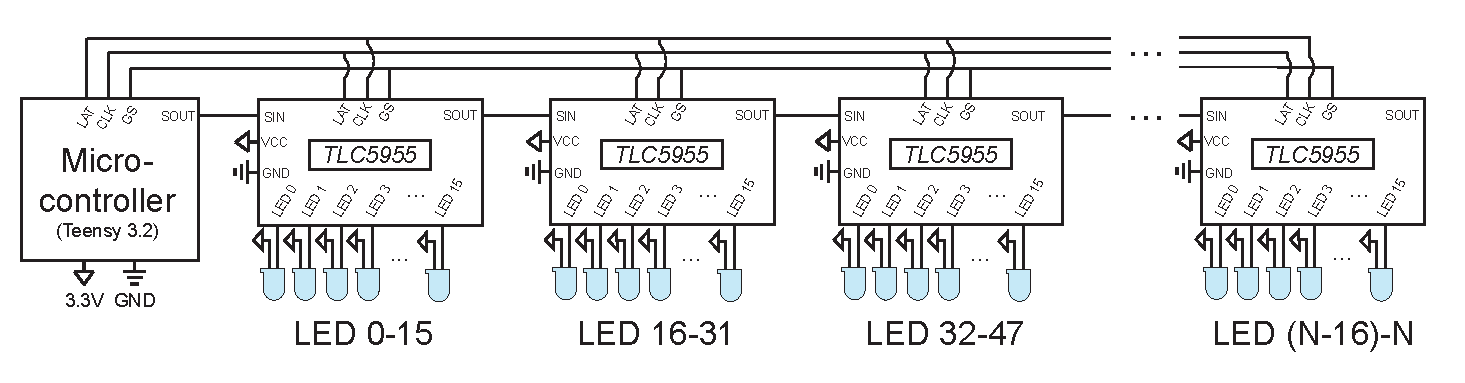
\includegraphics[width=\textwidth]{figures/fig_fabrication_slow_circuit.pdf}
    \caption{Circuit schematic for Quasi-dome device. A chain of up to 40 TLC5955 chips are connected in a daisy-chain configuration, having common Power (VCC), ground (GND), Grayscale-clock (GS), serial clock (SCLK), and latch (LAT) pins. These are controlled by a micro-controller upstream, which enables the control of up to $16 \times N_{chips}$ LEDs for $N_{chips}$ TLC5955 chips.}\label{fig:fabrication_dome_circuit}
\end{figure}

\section{Coded Illumination Devices for High-Throughput Microscopy}\label{sec:fabrication:highthroughput}

High throughput imaging using both strobed illumination and motion deblurring~\cite{raskar2006coded} requires light sources to be extremely fast compared to the domed devices presented in the previous section. In these systems, the sample is imaged and illuminated while being moved continuously by a mechanical motion stage, without stopping. A key parameter of a high-throughput illumination source is repetition rate, or the minimum pulse duration the source can provide. This time must be less than the time required for the sample to move one effective pixel size (pixel size divided by magnification) while being scanned. Mathematically, the source repetition period $T$ is related to the motion velocity $v_{motion}$, camera pixel size $\Delta$, and system magnification $M$ by the following relationship:

\begin{equation}
    T \leq \frac{\Delta}{Mv_{motion}}
\end{equation}

For practical systems (such as those described in Chapter~\ref{ch:highthroughput}), this threshold is on the order of micro-seconds, which is 3-4 orders of magnitude faster than the LED domes described in previous sections. For these applications, it was necessary to adopt very simple LED circuitry to avoid electronic speed limitations associated with dimming (using pulse-width modulation) and serial control of LED driver chips. As such, we adopt an extremely simple circuit, consisting of only a micro-controller and transistor, to control an arbitrary number of LED sources at very high speed, limited only by the clock-speed of the microcontroller. The drawback of this configuration is that only binary illumination is possible, but binary illumination is often optimal for both strobed and coded illumination (See Chapter~\ref{ch:highthroughput}).

For these applications, we developed two high-speed sources based on the same platform, one for high-throughput brightfield and quantitative phase imaging, and one for fluorescence imaging. The first device used 40 white (blue-phosphor) LED emitters (VAOL-3LWY4, VCC) controlled by four transistor circuits to modulate 4 quadrants of a circle. The intention of this design was to enable extremely fast brightfield (color) imaging, as well as quantitative phase imaging using DPC. The second used a single, high-power LED source (Thorlabs M470L3) modulated using a simple single-transistor circuit through the same micro-controller. Chromatic filters could be added to the illumination pathway and detection pathway to enable fluorescence imaging, and this device was compatible with a wide range of LED sources due to its modular design. Both of these devices used the same firmware as the micro-controller firmware, which was designed to be modular to accommodate various LED arrays~\cite{illuminate}. A schematic of this high-speed circuit is shown in Fig.~\ref{fig:fabrication_highthroughput_circuit}.

\begin{figure}
    \centering
    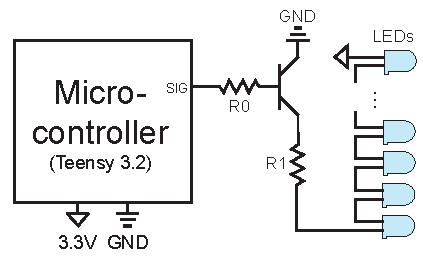
\includegraphics[width=0.4\textwidth]{figures/fig_fabrication_fast_circuit.pdf}
    \caption{Circuit schematic for fast LED driver circuit. A transistor (NPN type) is used to modulate a large current source for controlling many LEDs at once, which are connected in serial. Resistor R0 is normally set to 1K$\Omega$, and R1 is set such that the current is not too large based on the VCC voltage. This circuit enables micro-controller limited illumination updates, although it does not allow per-channel dimming and supports only binary illumination patterns.}\label{fig:fabrication_highthroughput_circuit}
\end{figure}

\clearpage

\section{Coded Illumination Devices for Portable Microscopy}
Optical microscopy is an important tool for disease screening and diagnosis throughout the world. Significant resources have been devoted to developing portable and affordable compact microscopes for remote clinical applications~\cite{Zhu2011, switz2014low, smith2011cell, maamari2013mobile,C4LC00010B,Vashist2014, steenblik2005lenses, cybulski2014foldscope, boppart2014point, Greenbaum17122014, mudanyali2010compact, tseng2010lensfree}.
Compact microscopes based on mobile phones, including CellScope~\cite{breslauer2009mobile, skandarajah2014quantitative}, have demonstrated that microscopy can be effectively performed outside of hospitals and diagnostic laboratories by minimally trained healthcare workers, that images can be transmitted for confirmation of diagnosis, and that phone-based computational analysis can be used to provide automated diagnosis.

\subsection{Computational CellScope}\label{sec:fabrication:ccs}
Here, a new variation of the CellScope microscope is demonstrated which incorporates recently developed techniques of computational illumination~\cite{Zheng2011, Tian14, zijiMulti} using the LED dome shown in Fig.~\ref{fig:fabrication_ccs_dome} to enable new imaging modalities, including darkfield, phase imaging and digital refocusing\footnote{This work was developed in close collaboration with Daniel Fletcher, Mike D'Ambrosio, and Neil Switz (Fletcher Lab, Bioengineering, UC Berkeley), as well as Lei Tian, Jared Rulison, Hurshal Patel, Nitin Sadras and Aditya Gande (Waller Lab, EECS, UC Berkeley).}. Using only the on-board processing power of a smartphone, our device implements quantitative phase recovery using DPC, as well as lightfield digital refocusing, so that a sample focus can be changed after the fact (without mechanically changing focus).

The flexibility and speed of the programmable LED array illuminator, as well as the lack of moving parts and low cost, make the hardware very amenable to modification as a CellScope attachment. In order for our device to be practically useful in the field, we have here enforced the requirement that all of our processing and control be performed on the smartphone, without use of a PC. Thus, the device can be field-deployable as a simple add-on to CellScope, requiring only a 7V-20V DC power source which could be adapted to many power sources, such as batteries, car batteries, or wall-outlets using commonly available adapters. In the following sections we detail the design and performance of the hardware and software of our new Computational CellScope device.

While our addition involves custom LED drive circuitry and a 3D printed structure, complexity was kept low to preserve the low-cost nature of CellScope. Part counts, cost and especially size may be further reduced in design-for-manufacture. The size of the illuminator could be reduced to essentially the dimensions of the dome itself, and cost could be comparable to the price of a modern smartphone, matching and improving upon the functionality of a full-size microscope at a fraction of the cost.

\begin{figure} [ht]
\begin{center}
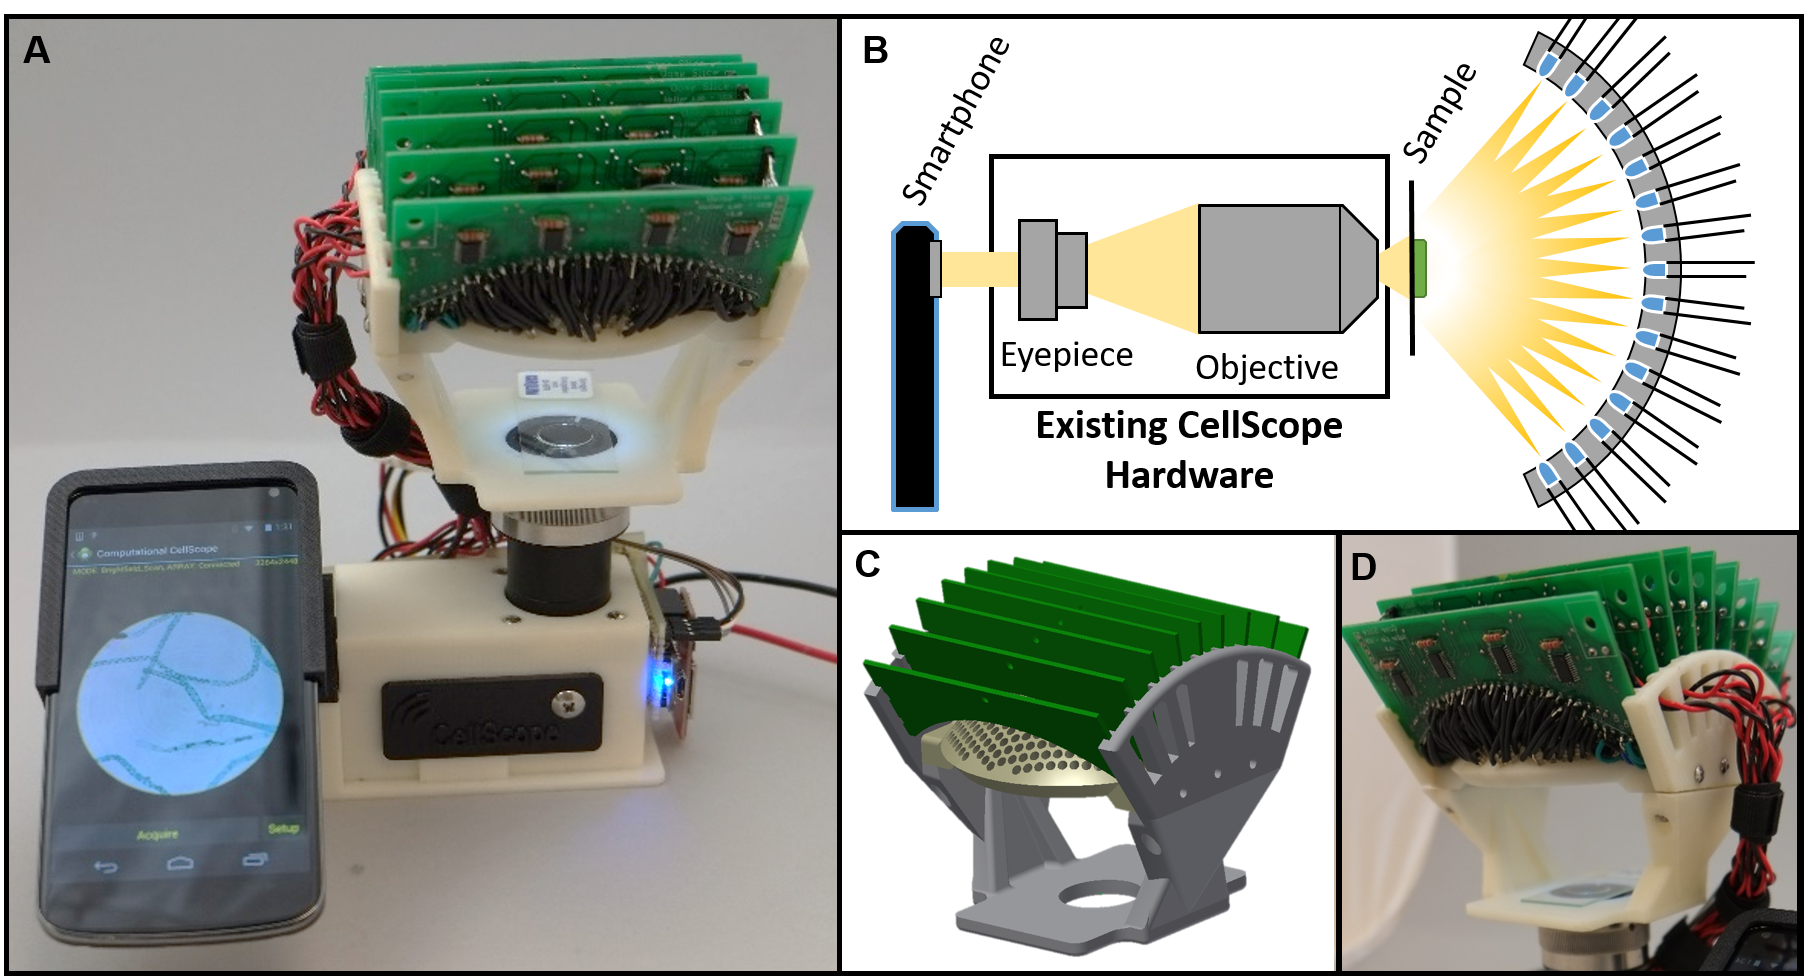
\includegraphics[width=0.8\textwidth]{figures/fig_ccs_system.png}
\end{center}
\caption {{Computational CellScope.} {a).} Device observing a sample using a Nexus 4 smartphone. {b).} Optical schematic of the CellScope device with our custom-made domed LED illuminator. {c).} CAD assembly of the dome. {d).} Assembled dome and control circuitry.}
\label{fig:fabrication:device}
\end{figure}

% Contrast method comparison figure
\begin{figure}
\begin{center}
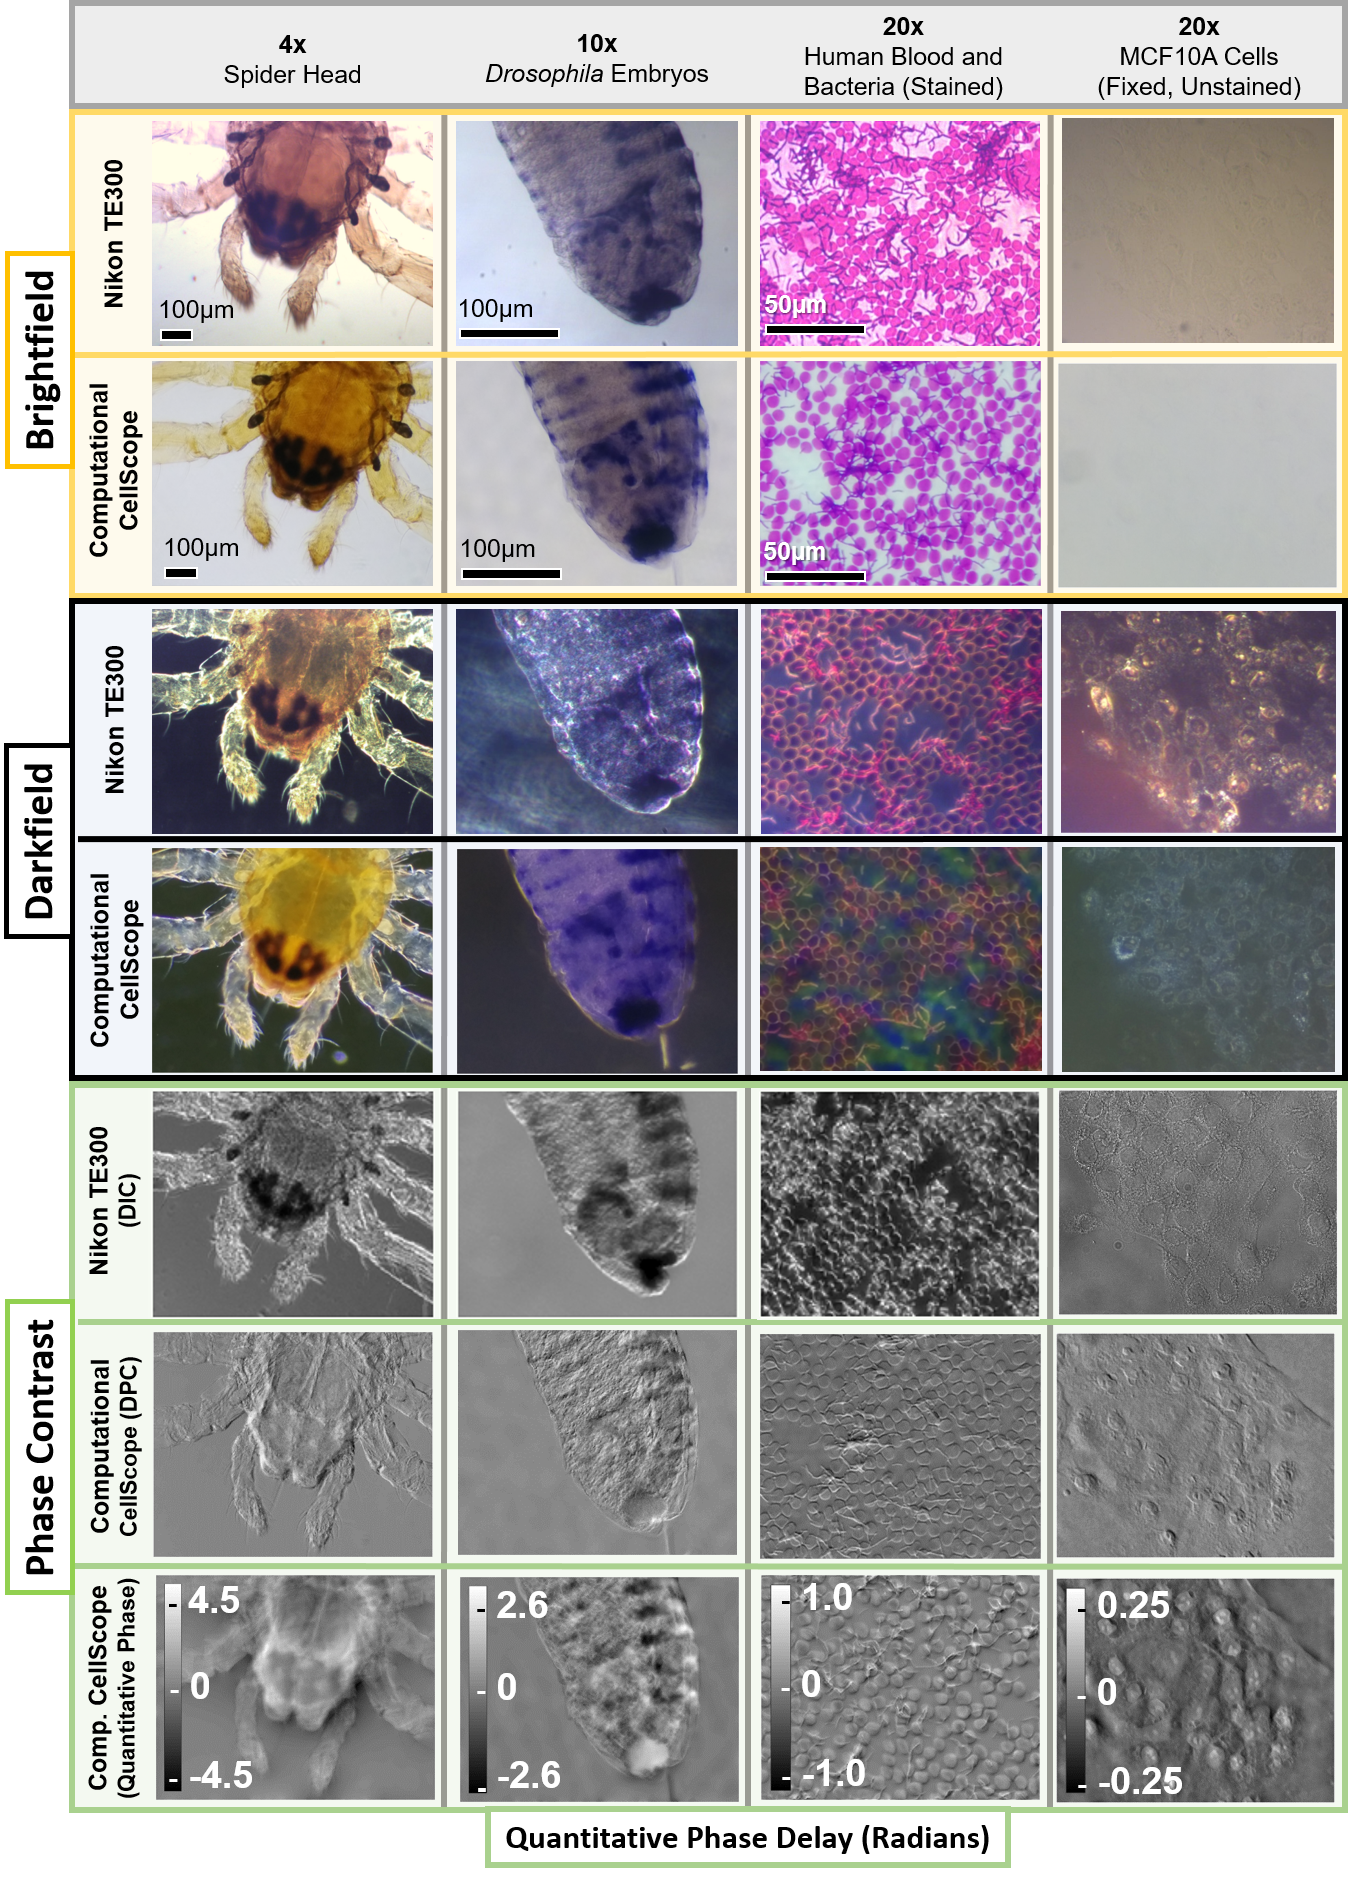
\includegraphics[width=0.6\textwidth]{figures/fig_ccs_mosaic.png}
\end{center}
\caption {{Image results compared to a standard microscope.} Computational CellScope acquires brightfield and darkfield images of similar quality to a standard upright microscope (Nikon TE300) without the use of hardware inserts. Additionally, it enables phase imaging using Differential Phase Contrast (DPC), which contains similar information to standard phase contrast imaging, and can be inverted to obtain quantitative phase of the sample (bottom row). Differences in color shades are caused by the relative differences in hue of the halogen lamp and the white LEDs. Note the additional dark features in DIC results, as compared to DPC, illustrating mixing of phase and absorption information in DIC. In the right-most column, we show images for an unstained transparent sample, illustrating the utility of phase imaging methods for label-free imaging.
}
\label{fig:fabrication:contrastcomparison}
\end{figure}

\subsection{Multi-Contrast Imaging}
To achieve brightfield, darkfield and phase contrast simultaneously, we time-multiplex images taken with different LED patterns and post-process them on the smartphone to synthesize pseudo-real-time multi-contrast imaging, as in~\cite{zijiMulti}. Brightfield images correspond to illumination by LEDs that lie within the cone of angles described by the objective numerical aperture (NA). Darkfield images are obtained by illuminating the sample from angles beyond the angular acceptance of the objective (Fig.~\ref{fig:fabrication_ccs_dome}a)~\cite{Zheng2011}. Since different objectives have different NA, one must specify in the software which objective is being used, with larger NA corresponding to a larger brightfield region of LEDs. Our dome is designed to enable darkfield contrast for any objective of NA$<0.62$, roughly corresponding to a typical 40$\times$ objective.

Phase contrast can be achieved in a single-shot image by any asymmetric illumination pattern~\cite{kachar1985asymmetric,Dodt01101999}. Here, we choose to employ a differential phase contrast (DPC) scheme~\cite{Hamilton1984a,mehta2009quantitative,Tian14,ford2012phase}, which requires two images having complementary illumination patterns, because it gives good phase contrast at all spatial frequencies and can be quantitatively interpreted as the gradient of sample phase. The method involves sequentially illuminating the sample with the two opposite halves of the brightfield circle while capturing an intensity image for each. For example, one may first take an image, $I_\mathrm{R}$, with only the right half of the LEDs on and then a second image, $I_\mathrm{L}$, with only the left half of LEDs on (see Fig.~\ref{fig:fabrication_ccs_dome}b). The two images are processed as follows to obtain brightfield and phase contrast:

\begin{equation}
I_{\mathrm{BF}}=I_\mathrm{L}+I_\mathrm{R}, \qquad I_{\mathrm{DPC}}= \frac{I_\mathrm{L}-I_\mathrm{R}}{I_\mathrm{L}+I_\mathrm{R}},
\label{IBF}
\end{equation}

\noindent where $I_{\mathrm{BF}}$ is the brightfield image and $I_{\mathrm{DPC}}$ is the phase contrast image. Since the LEDs are mutually incoherent, adding the two images gives an equivalent brightfield image and subtracting them produces phase contrast, due to asymmetric clipping in Fourier space. The intensity of the DPC image can be shown to be approximately proportional to the first derivative of phase along the direction of illumination asymmetry~\cite{Hamilton1984a}, and different axes of rotation can be programmed by changing the LED array pattern accordingly. Typically, we capture an additional two images in order to compute both the left-right and top-bottom phase derivative results representing both orthogonal directions. DPC images are qualitatively similar to Differential Interference Contrast (DIC); however, the latter is not a quantitative method. To obtain quantitative phase from DPC images, we solve the inverse problem~\cite{mehta2009quantitative,tian20153d} using a simple deconvolution in Fourier space. Results for all of the contrast modalities are shown in Fig.~\ref{fig:fabrication:contrastcomparison}.

Thus, by acquiring four half-brightfield images and a single darkfield image for each time point, we can synthesize brightfield, darkfield, and phase contrast modes in near real-time. Users have the option of saving and post-processing time-multiplexed frames or viewing a live multi-contrast display of the sample, though display speed is significantly faster in the latter case due to limited file write speeds on the smartphone. We developed an application to stream these four contrast modes size-by-side while updating each frame sequentially as the illumination pattern cycles through the different patterns (Fig.~\ref{fig:fabrication:android}b). The user may touch any of the four images for a live full-screen display of that contrast mode only, and the illumination pattern cycle will update to reflect this.

Some image results for each of the contrast modes are shown in Fig.~\ref{fig:fabrication:contrastcomparison}, using different objective magnifications and samples. For comparison, we show the same samples imaged in a commercial inverted microscope with traditional hardware. Darkfield was obtained by using a Ph3 condenser aperture in combination with objectives having NA smaller than the sine of the half-angle of the Ph3 annulus inner diameter. Since DPC is not currently commercially available, we instead compare our DPC phase contrast images to (similar-appearing) DIC. Both provide images whose contrast is related to the first derivative of phase along a single direction; however, DIC mixes absorption and birefringence information with phase, so that dark features in the image may result from either absorption of the sample or phase contrast interferences. In the DPC images, on the other hand, the image is related purely to the sample phase distribution (see Fig.~\ref{fig:fabrication:contrastcomparison}), which can be inverted to reveal quantitative phase, as shown in the bottom row. Provided in a portable package, these multi-contrast video and streaming methods have the potential to allow clinicians to view a sample with three separate contrast methods at once, enhancing the information available for diagnosis and disease discrimination.

\subsection{Digital Refocusing}
For thick samples, our system can capture a different sequence of images in order to recover 3D images and enable digital refocusing. In this case, we sequentially capture images for each of the LEDs in the brightfield region. The resulting dataset is similar to limited angle tomography with many angles, which provides depth sectioning from angular information~\cite{Kak:1988fk}. For simpler processing more amenable to mobile phone programming, we use a lightfield approach here ~\cite{Ng2005,Zheng2011}. This involves a simple shift-and-add algorithm to digitally refocus the image to different axial ($z$) planes. We calculate the digitally refocused intensity image at a distance $\Delta z$ away from the physical focus plane as:
\begin{equation}
I^{\Delta z} = \sum_{\text{all brightfield LEDs}}I_i(x+\Delta z\tan{\theta_x}, y+\Delta z\tan{\theta_y}),
\label{I_refocus}
\end{equation}
where $I_i$ denotes the intensity image for the $i^{\text{th}}$ LED, shifted according to its angle of illumination at the sample $(\theta_x,\theta_y)$ and the desired refocus distance $\Delta z$.

The number of individual LEDs making up the brightfield region roughly determines the number of depth planes that can be accurately reconstructed, and the range of illumination angles determines the axial resolution of the 3D result. Since a separate image is taken for each illumination angle, both acquisition and processing time are a function of the numerical aperture of the objective, as illustrated in Fig.~\ref{fig:fabrication:android}. Acquisition speed was primarily limited by the time required to save an image to the smartphone's flash memory at full resolution (8 Megapixels on the Nexus 4). This is important because data acquisition remains fast, while processing can occur in the background. Using the same dataset, we can also calculate 3D phase contrast images by digitally refocusing the two halves of the brightfield region separately~\cite{Tian14}. It is expected that this mode of imaging intensity or phase in 3D with no moving parts will give better diagnostic information for thick samples. Alternatively, it could be used for correcting misfocus, obviating the need for automatic axial translation or automated focus adjustment in long time-lapse studies.

% Digital refocus results figure
\begin{figure}
\begin{center}
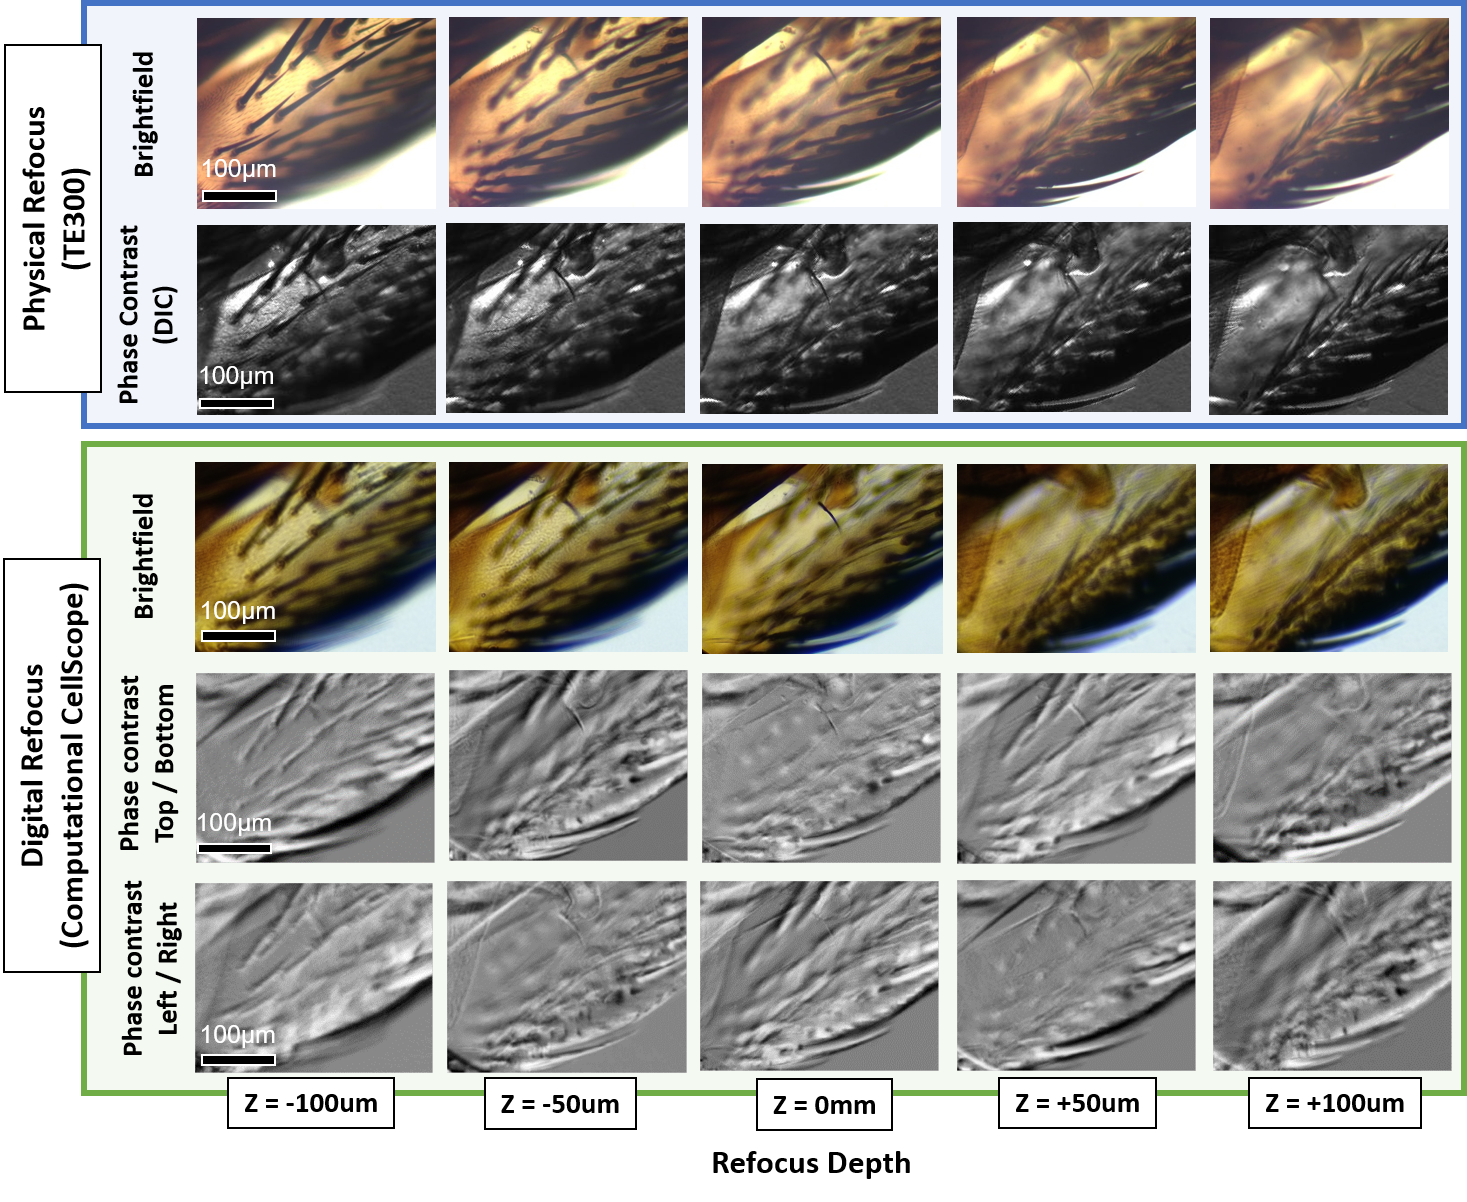
\includegraphics[width=\textwidth]{figures/fig_ccs_refocus.png}
\end{center}

\caption { {Digital refocusing on the Computational CellScope.} Comparison of digital refocusing to physical refocusing on a commercial microscope (Nikon TE300) of a house fly wing sample (AmScope PS200) with a 10$\times$ objective. Digitally refocused phase contrast images are also computed for both vertical and horizontal phase derivatives at different focus depths.}

\label{fig:fabrication:digrefocus}
\end{figure}

Results are shown in Fig.~\ref{fig:fabrication:digrefocus} for digitally refocused images as compared to physically refocused images on an inverted microscope (Nikon TE300), both with a 10$\times$ objective (0.25 NA). The phase contrast images show the first derivative of phase along both the vertical and horizontal directions, calculated from the same dataset using only the green color channel. The algorithm successfully refocused features across 400$\mu$m depth of field, limited by object thickness. Our refocusing achieves an axial resolution of approximately 5$\mu$m within $\pm50\mu$m of physical focus position but degrades approximately linearly with increasing refocus distance~\cite{Tian14}. Processing time is approximately 1.5 minutes per depth slice for a 10$\times$ objective.

% Application Timing and Screenshot figure
\begin{figure}
\begin{center}
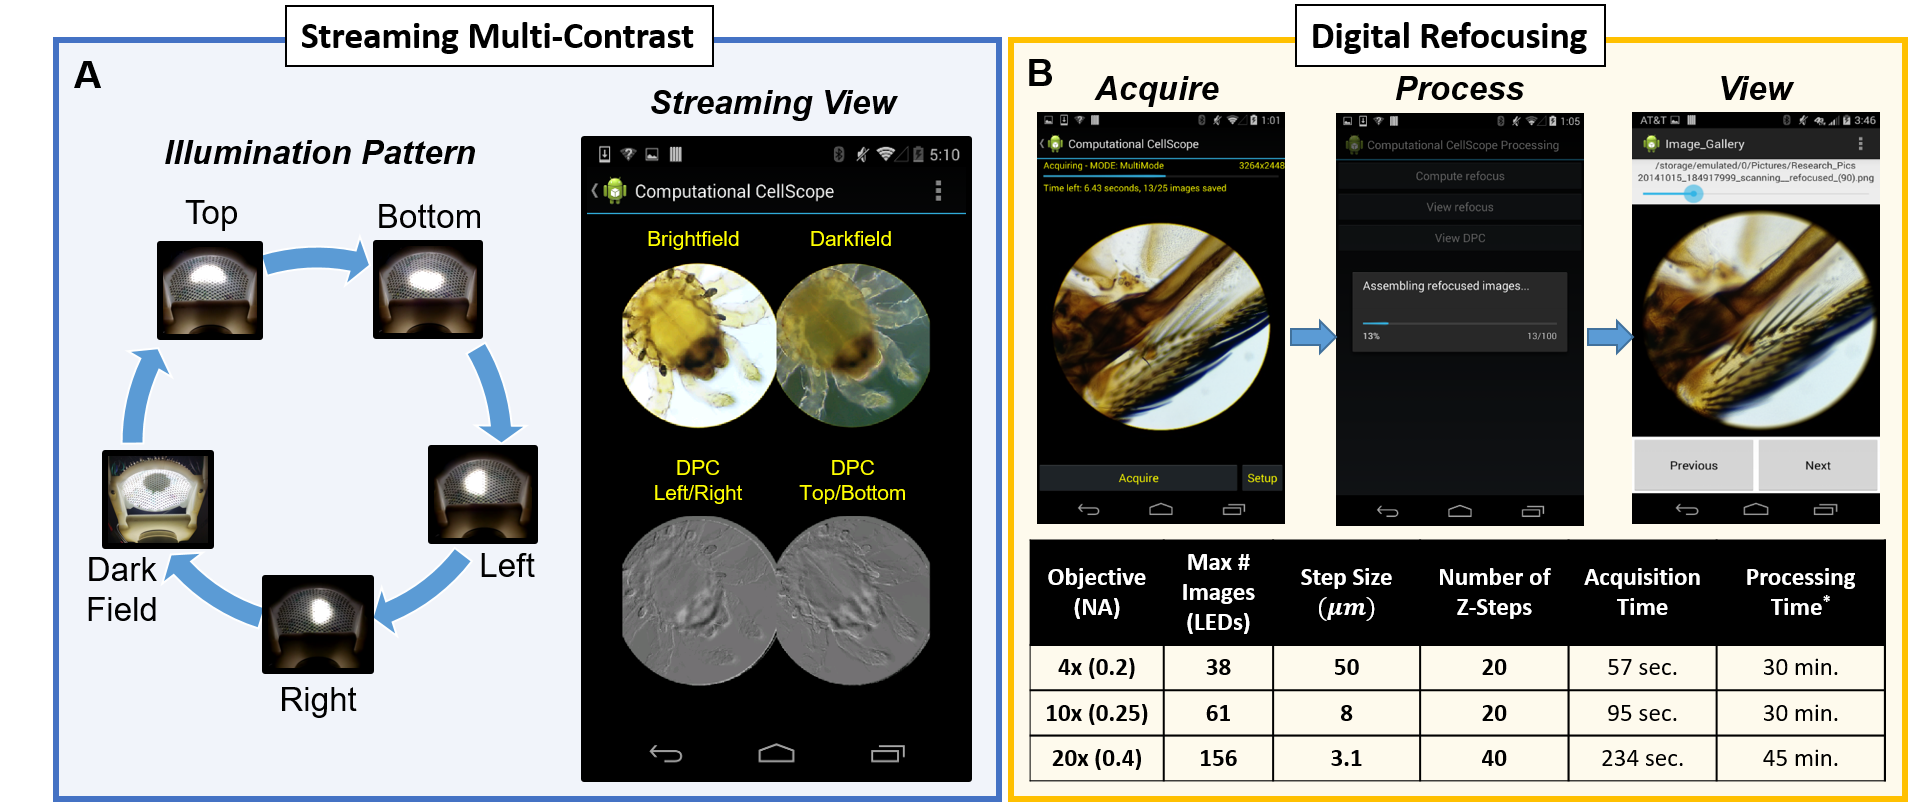
\includegraphics[width=\textwidth]{figures/fig_ccs_app.png}
\end{center}
\caption {{Android Application Workflow.} {a).} Schematic of streaming multi-contrast LED patterns. Here we vary the LED pattern in time and acquire and process images on the smartphone, producing a streaming multi-contrast display of a sample without any further post-processing. The user can touch any image to zoom in and stream an individual image. Total cycle time is 2.3 seconds.
{b).} Overview of workflow for digital refocusing mode. Table shows example processing and acquisition times for a typical dataset reconstruction. Axial Resolution is determined by the range of illumination angles sampled (defined by the objective NA). The number of z-steps were chosen such that refocus blur does not exceed 20 pixels. Processing and acquisition time can be reduced by selecting fewer refocus planes or by sparsely sampling LEDs, trading axial resolution for faster acquisition time.}

\label{fig:fabrication:android}
\end{figure}

\subsection{Acquisition Software and Processing}
It has previously been shown that using a smartphone as a microscope poses unique challenges intrinsic to the phone software~\cite{skandarajah2014quantitative}. Smartphone cameras may only allow minimal quantitative control over standard imaging parameters (e.g. focus, exposure, gain), opting for opaque automatic algorithms that simplify the user experience. To circumvent these restrictions, we wrote a custom Android application that attempts to achieve the optimum imaging characteristics with our coded illumination configuration. The software application also initiates and handles the Bluetooth connection to the domed array, enabling synchronized acquisition and array control through the standard Android API. Array control is thus transparent to the end-user, requiring them to simply pair the phone with the illuminator and press a connect button to initiate a Bluetooth connection. Our application was developed specifically for the Android platform and will be compatible with any phone running Android OS version 4.0 or later. However, our algorithms were developed using the OpenCV Library, which is cross-platform for iOS (Apple, Inc.) and other operating systems. Thus, most of our application code is portable to other smartphone platforms with moderate development effort. A screenshot of the acquisition and processing are shown in Fig.~\ref{fig:fabrication:android}. The user may choose to collect and synthesize any or all of darkfield, refocused brightfield and DPC images.

In our application, images were acquired using the standard Android API, which does not provide an interface to set explicit exposure times, but supports only continuous auto-exposure with predefined exposure offset values. To circumvent this issue, we included a short pre-illumination sequence before each dataset acquisition to lock exposure at the appropriate value and enforce the requirement that equal numbers of LEDs be chosen for each half-circle. Finally, we incur significant latency between the camera shutter and the availability of the frame to our application within the API, due to post-processing algorithms integral to the phone and performed in the background (e.g. white balance and demosaicing). This severely limits our acquisition speeds, which will likely be improved in newer versions of Android that allow finer camera control through the API. Apple iOS offers a different camera API that may also offer improvements in acquisition speed.

Data post-processing was performed in a standalone Android app, where image stacks were loaded and processed on the phone. We employ a number of functions of the OpenCV Imaging library for Android to perform most of our computation. Individual DPC images are computed in less than a second, as demonstrated in our multi-contrast view mode. Digitally refocusing an image into 21 depth planes ($\pm$100 $\mu$m range with 10 $\mu$m sectioning) requires approximately 30 minutes of processing time, but the resulting 3D image stack can be interacted with in real-time; all other computational imaging results are much faster ($\sim$0.43 frames/sec). The long processing time is attributed to frequent loading and saving to the smartphone's internal storage. We note that significant improvement in processing speeds for all of our algorithms is possible through implementation using the Android NDK and is also expected as phone computational power increases with each product generation. These performance metrics were calculated on a Nexus 5 smartphone (LG Electronics) and may vary on other devices.

\section{Summary}
In this chapter, we presented several examples of the fabrication and design process for coded illumination devices. These devices are each the result of many design iterations which incorporate the joint design of hardware and software - a key paradigm of computational imaging. The recent development and commercialization of 3D-printing has enabled rapid prototyping of optical devices, enabling the fabrication and iteration of domed LED illuminators (As show in in Section~\ref{sec:fabrication:ccsdome}). However, due to practical fabrication limitations, we found that reverting to more standardized printed circuit board (PCB) approach (Section~\ref{sec:fabrication:quasidome}) enabled significantly improved manufacturability without significant performance degradation, enabling more rapid dissemination of domed LED illuminators around the world. We also developed coded illumination prototypes with much higher temporal illumination resolution for high-throughput imaging (Section~\ref{sec:fabrication:highthroughput}), which required different design decisions to be made to accommodate rapid temporal coding of LEDs. Finally, in Section~\ref{sec:fabrication:ccs} we described a complete coded illumination solution for portable microscopy using a 3D-printed domed illuminator. This device enabled portable implementations of qualitative microscopy (darkfield and brighfield), quantitative phase imaging using DPC, and 3D digital refocusing of thick samples, all using only the existing smartphone and the addition of our domed illuminator. This device demonstrates how flexible and amenable coded illumination devices can be through example; future work could demonstrate an improved prototype which is fully field-ready in terms of robustness and flexibility and could enable new applications such as high-throughput imaging and fluorescence imaging.
